%% Use the "review" option when submitting for review.
%% Removing the "review" option will switch the
%% manuscript to a two-column layout.
%%
%% Use option "jog" for submissions to the Journal of
%% Glaciology; use "aog" for submission to the Annals
%% of Glaciology.
% \documentclass[review,aog]{igs}
%\documentclass[,aog]{igs}
\documentclass[aog]{igs}
\usepackage[utf8]{inputenc}
\usepackage{natbib}
\usepackage{mathabx}
\usepackage{graphicx}
\usepackage{siunitx}
% if you really must have numbered sections, remove
% the % from the beginning of the following command
% and insert the level of sections you wish to be
% numbered (up to 4):

% \setcounter{secnumdepth}{2}

\jourvolume{12}
\jourissue{1}
\jourpubyear{2024}

\begin{document}

\title[Floe-scale sea ice motion]{Characterizing the Summer Marginal Ice Zone in the Greenland Sea Through Floe-Scale Sea Ice Observations}

\author[Watkins and others]{Daniel M. WATKINS,$^1$
  Ellen M. BUCKLEY,$^2$ Minki KIM,$^1$ 
  Monica M. WILHELMUS$^1$}

\affiliation{%
$^1$Center for Fluid Mechanics, Brown University, Providence, RI, USA\\
$^2$Department of Earth Science \& Environmental Change, University of Illinois Urbana-Champagne, Urbana, IL, USA\\
  Correspondence: Monica M. Wilhelmus 
  \email{mmwilhelmus@brown.edu}}

\begin{frontmatter}
\maketitle

\begin{abstract}
Sea ice motion in the marginal ice zone (MIZ) is inherently multi-scale. 
The spatial and temporal scales of motion are influenced by the relationship between the sizes of individual ice floes and the scales of winds and currents.
Joint observations of the floe size distribution (FSD) and sea ice motion are necessary to develop and validate models of the MIZ. 
However, such observations are rare.
We present observations of floe-scale Lagrangian sea ice motion and rotation in the East Greenland MIZ spanning the spring-to-summer transition for years 2003-20.
The observations are derived from moderate-resolution optical imagery using the Ice Floe Tracker (IFT) algorithm and consist of floe shapes, geometric properties, and trajectories.
We investigate the seasonality of the FSD, links between floe size, motion, and rotation, and length scale dependence of deformation. 
The IFT observations are compared to large-scale sea ice motion from the NSIDC Ice Motion Vectors product and to discrete element model simulations.
We find that drift anomalies approximately follow an exponential distribution. 
Both the IFT observations and model results indicate that drift and rotation variability depend on the floe size. 
These observations provide a new avenue for sea ice model development and validation in the MIZ.

\end{abstract}
\end{frontmatter}

\section{Introduction}
% Why the floe scale matters
The size of an individual plate of ice--the \emph{floe scale}--is foundational to sea ice dynamics in the marginal ice zone (MIZ).
The relationship between the floe scale and the spatial scales of atmospheric and oceanic motion is important for understanding coupled interactions, as stresses from the atmosphere and ocean are integrated across the surface of the floe \citep{brenner2023_ScaleDependentAirSea,
gupta2024_EddyInducedDispersion,
kim2024_CharacterizationSea}. The spacing between floes and the range of floe sizes in an area, characterized by the sea ice concentration (SIC) and the floe size distribution (FSD), respectively, strongly affect air-ocean fluxes, wave-ice interactions, and floe-floe interactions \citep{Mcnutt2003, loose2014_ParameterModel, wenta2018_InfluenceSpatial, horvat2022_FloesMarginal, herman2022_GranularEffects, manucharyan2022_SpinningIce, brenner2024_ScalingSimulations}.
Thus, joint observations of floe shapes and motion are needed to characterize MIZ sea ice dynamics.

Spatial and temporal variability in ice motion is directly related to the FSD and SIC \citep{overland1995_HierarchySea, dumont2022_MarginalIce,
herman2022_GranularEffects}.
The FSD is constantly evolving as floes either become larger due to pieces of ice interlocking, rafting, ridging and fusing, or smaller  due to fracture and melt \citep{zhang2015_SeaIce, horvat2016_InteractionSea, bateson2020_ImpactSea, roach2024_PhysicsSeasonal}.
The tight coupling between the seasonally evolving FSD, mesoscale and submesoscale ocean currents, waves, and wind stress in the MIZ results in complex sea ice motion patterns with low spatial correlation (meters to kilometers) and short temporal scales (hours to days, \cite{hakkinen1987_FeedbackIce, johannessen1987_MesoscaleEddies,
johannessen1987_IceEdgeEddies, feltham2005_GranularFlow,  cole2017_IceOcean, watkins2023_EvidenceAbrupt}).

This complexity poses a challenge for sea ice observation and modeling.
Sea ice is motion is routinely monitored through drifting buoys and from processing remote sensing imagery \citep{webster2022_ObservingArctic, gerland2019_EssentialGaps, sandvenSeaIceRemote2023}.
The physical processes that can be resolved by a particular sea ice observation system are constrained by the spatial resolution and acquisition frequency.
Outside dedicated experiments where multiple observation sources are merged \citep[][e.g.]{uttal2002_SHEBA, hwang2017_WintertosummerTransition, rabe2024_MOSAiCDistributed}, few observation sources exist that jointly observe ice dynamics and floe properties. 

Buoys track the motion of individual ice floes with high precision. 
At large scales (greater than 100 km), operational buoy deployments through the International Arctic Buoy Program (IABP, \cite{rigor2008}) provide long-term coverage. 
Due to the difficulty and expense of deployment, this data is spatially and temporally sparse, particularly in the MIZ \citep{gerland2019_EssentialGaps, brunette2022_NewStatedependent}.
In addition, information on sea ice properties from buoys is limited to point-wise measurements.
Hence the representativeness of a buoy observation in space must be estimated, for example, through collation with other sensors.

Remote sensing observations from satellites and aircraft enable observation of sea ice properties across large spatial regions.
Ice motion is estimated from satellite imagery by tracking the displacement of groups of pixels, for example through maximum cross-correlation \citep{girard-ardhuin2012_EnhancedArctic, lavergne2010_SeaIce}.
For such methods, the motion vectors produced represent an area-average within the spatial footprint used by the correlation algorithm.
In the pack ice, where spatial correlation is high, the region within the footprint moves coherently and displacement estimates can have high confidence. However, in the MIZ, the same footprint may include thousands of jostling floes and uncertainty in remote sensing motion retrievals tends to be highest in these areas \citep{sumata2014_IntercomparisonArctic, gui2020_ValidationRemotesensing}.
Moreover, many products are only available seasonally, with few products providing estimates of motion during the summer melt season due to the presence of liquid water at the snow and ice surface \citep{lavergne2010_SeaIce, girard-ardhuin2012_EnhancedArctic}. 
Thus the representativeness, availability, and uncertainty of remote sensing-derived ice motion vectors varies spatially and temporally.

In contrast to sea ice motion, the FSD is not routinely measured, though standard operational ice charts do include information on predominant floe size categories \citep{dedrickUSNationalNaval2001, afanasyevaAARIMethodologySea2019}. 
To date, knowledge of the properties and variability of the FSD comes through individual studies.
Observation of the sea ice FSD from airborne remote sensing imagery dates back to \cite{rothrock1984_MeasuringSea}.
Noting an approximately linear FSD probability density function (PDF) in log-log space, they suggested characterization of the FSD via a power law with the form
\begin{linenomath*}
\begin{equation}
    p(x) = cx^{-\alpha} \label{powerlaw}
\end{equation}
\end{linenomath*}
where $x$ is a measure of floe size, $c$ is a normalization constant and the parameter $\alpha$ is the slope of the power law distribution on a log-log scale.
Numerous methods and image types have been taken to characterize the FSD \citep{pagetDeterminingFloesizeDistribution2001,  toyota2006_CharacteristicsSea, hwang2013_IntercomparisonSatellite}.
Measured FSD properties (and methods) vary substantially across studies \citep{stern2018_ReconcilingDisparate}, often showing a clear departure from Eq. \ref{powerlaw}. 
Note that the form of Eq. (1) is an empirical, not theoretical result \citep{herman2010_SeaiceFloesize}, and distinct mechanisms governing FSD evolution may lead to other forms of the FSD PDF \citep{montiel2022_TheoreticalFrameworka, mokus2022_WavetriggeredBreakup}.

Development and validation of models capable of simulating small-scale sea ice variability requires observations of sea ice across scales.
Traditional models of sea ice dynamics and thermodynamics rely on a continuum approximation. Most current coupled climate models use a form of the viscous-plastic or elastic-viscous-plastic rheology (\cite{Hibler1979}, \cite{hunke1997_ElasticViscous, tandon2018_ReassessingSea}).
Such models successfully reproduce many aspects of large-scale sea ice dynamics and thermodynamics (\cite{hutter2018_ScalingProperties, zhang2021_SeaIce}), but are not well suited to the scales of motion observed in MIZs \citep{herman2022_GranularEffects}.
Observations of scale dependence in sea ice deformation using SAR-derived Lagrangian ice trajectories \citep{Marsan2004, Stern2009} have motivated the development of alternative approaches, including the elastic anisotropic plastic \citep{tsamados2013_ImpactNew, heorton2018_StressDeformation} and brittle rheologies \citep{Girard2011, rampal2016_NeXtSIMNew, olason2022_NewBrittle}.  Similar scale dependence has been described in buoy data by, e.g., \cite{Rampal2008}.
Reconciling the levels of model complexity needed for large-scale climate simulations, local-scale forecasting, and process-level investigations of sea ice physics remains an active area of debate \citep{blockleyFutureSeaIce2020}.

The inclusion of FSD parameterizations in continuum models is seen as a potential path forward for better simulation of small scale thermodynamic and dynamic sea ice processes and wave-ice interactions in continuum models \citep{zhang2015_SeaIce,horvat2015_PrognosticModel, roach2018_EmergentSea, bateson2020_ImpactSea}.
Alternatively, discrete element models (DEMs) include the effects of the FSD on ice motion either explicitly (disks, polygons, e.g. \cite{gupta2024_EddyInducedDispersion, damsgaard2018_ApplicationDiscrete, brenner2023_ScaleDependentAirSea,manucharyan2022_SubZeroSea}) or implicitly through bonded particles \citep{astromHighResolutionFractureDynamics2024}.
The high computational cost of DEMs has historically limited their applicability to large-scale coupled Earth system models.

In this article, we present observations of floe-scale sea ice motion derived from optical satellite imagery. We focus on the Fram Strait and East Greenland ice tongue due to its importance as a connection between the Arctic and the world oceans \citep{smedsrud2017_FramStrait, sumata2022_UnprecedentedDecline}. 
In addition, the presence of sharp gradients in the ocean currents and distinct mesoscale features affecting the ice dynamics \citep{manley1987_EffectsSub, kozlov2021_EddiesMarginal, morozov2023_EddiesArctic, watkins2023_EvidenceAbrupt} make it an ideal testbed for measuring complex, small-scale sea ice dynamics.
Our observations aim to fill a major observational data gap for sea ice dynamics in the summer MIZ.
Floe shapes detected by the algorithm enable analysis of the sampling variability and seasonality of the FSD.
The observations are presented alongside the results of a discrete element sea ice model simulation showing the effects of mesoscale and submesoscale eddy forcing on sea ice rotation and drift variability.
We emphasize the effects of floe size and averaging area on sea ice motion, including effects of an evolving floe size distribution (FSD), proximity of the sea ice edge, and the presence of a rich upper ocean eddy field.

\section{Data}
\subsection{Sea ice segmentation and tracking}
We obtain measurements of floe-scale sea ice motion derived from moderate resolution optical satellite imagery using the Ice Floe Tracker (IFT) algorithm \citep{lopez-acosta2019_IceFloe}. The study region covers the area northeast of Greenland from the Fram Strait in the north to Scoresby Sound in the south (Fig. \ref{fig:study_region}, green box). The dataset consists of segmented satellite imagery, floe shape statistics, and derived floe trajectories. We first describe the source data, algorithm, and post-processing routines, then summarize the contents of the dataset. The full dataset is available at the Brown Digital Repository \citep{lopez-acosta2024_FramStrait}.

\begin{figure*}[!ht]
\centering{\includegraphics[width=89mm]{fig01_study_region.pdf}}
\caption{Map of the study region (green box) and extent of image details for subsequent figures (solid orange, solid purple, and dashed pink boxes). Blue lines show the mean April sea ice extent for each year 2003-20, while pink lines show the September mean.}
\label{fig:study_region}
\end{figure*}

\subsubsection{Satellite imagery}
We acquired daily 250-m resolution true color (bands 1-3-4) and false color (bands 7-2-1) mosaic imagery from the Moderate Resolution Imaging Spectroradiometer (MODIS) using the NASA Worldview Snapshots utility (Fig. \ref{fig:algorithm}a, b). 
Two images are used each day, corresponding to the daytime overpasses of the Aqua and Terra satellites.
Data are provided on a North Polar Stereographic grid.
As imagery is only labeled with the date, we use the Satellite Overpass Identification Tool \citep{hatcher_simon_2022_6475619} to identify the precise overpass time for each image for use in ice motion calculations.
We focused on the spring and summer months (April 1 to September 15) to ensure consistent illumination, and cover years 2003-20. Sea ice in the region has a large seasonal cycle and significant year-to-year variability. Blue and red lines in Fig. \ref{fig:algorithm} mark the April and September mean sea ice extent for each year. 
The end-of-season ice extent exhibits greater year-to-year variability than winter extent.

\begin{figure*}[!ht]
\centering{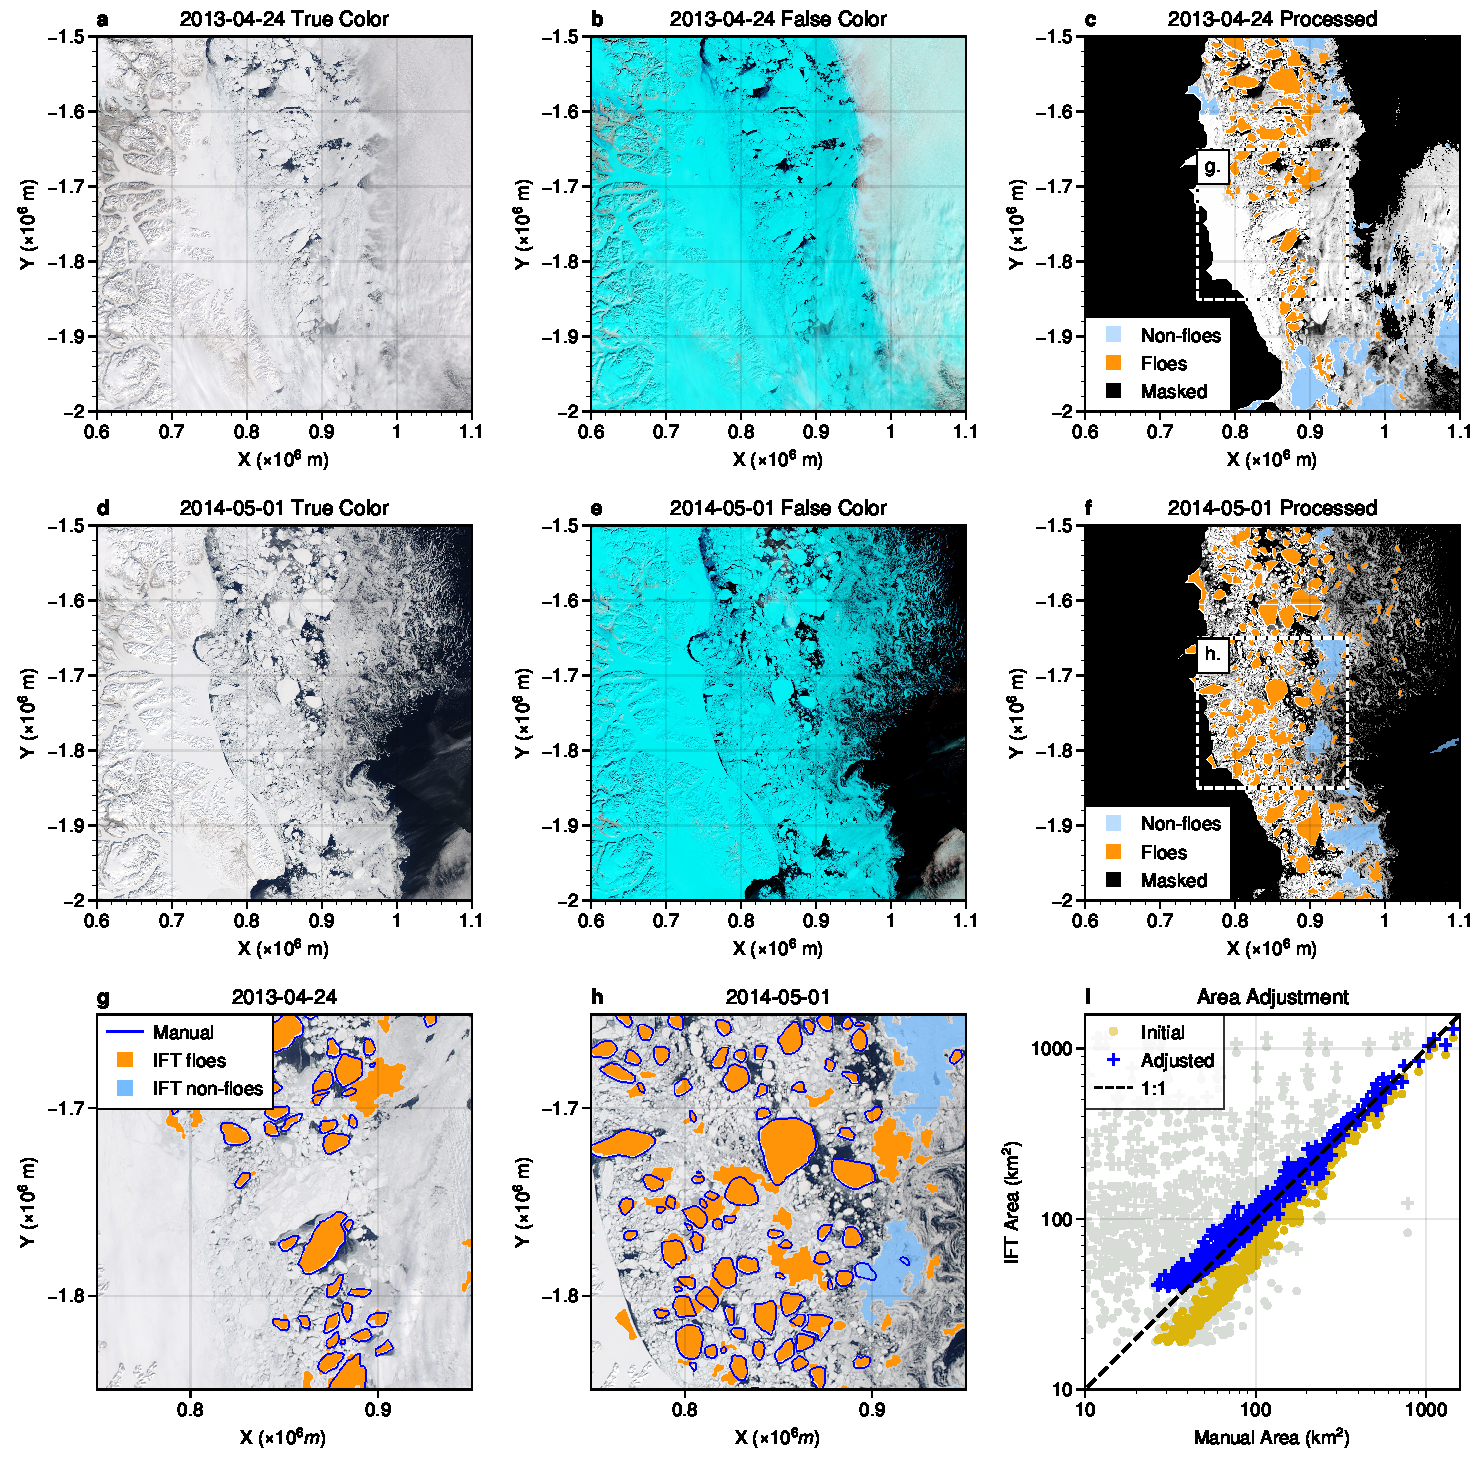
\includegraphics[width=179mm]{fig02_algorithm_example.pdf}}
\caption{Top: True color (a), false color (b), and processed (c) images for 2014-05-01 from the \textit{Aqua} satellite. In the processed image, masked regions (including the dilated land mask and the cloud mask) are black. Candidate segments are labeled as either floes (orange) or non-floes (light blue); non-floes are discarded in the final product. Bottom: Details of \textit{Aqua} truecolor images from (d) 2013-04-24 and (e) 2014-05-01 with overlaid IFT segmentation results, with objects labeled as floes marked in orange and discarded objects in light blue. Manually identified floe boundary for the true positive floes are shown in dark blue. Panel (f) shows the area of manually labeled well-segmented objects versus IFT results for the dates shown in (d) and (e) initially (gold) and after area adjustment (blue). Objects with poor correspondence to manual floe labels are marked in gray. The one-to-one line is shown in black. Image locations are shown in Fig. \ref{fig:study_region}.} 
\label{fig:algorithm}
\end{figure*}

\subsubsection{Gridded sea ice data products}
We use the NSIDC Daily Ice Motion Vectors data product to estimate the time-average sea ice drift at moderate to large scales \citep{tschudi2020_EnhancementSea}.
This product merges ice motion estimates from passive microwave imagery, buoys, and from reanalysis wind data.
The motion vectors are provided on a 25-km grid at daily resolution.
Note, however, that the effective resolution is generally coarser than this, as the source satellite motion resolution is 37.5-75 km \citep{tschudi2020_EnhancementSea}. 
We use sea ice concentration (SIC) from the
{NOAA/NSIDC} Climate Data Record (CDR) of Sea Ice Concentration.
This product combines SIC estimates from the NASA Team and NASA Bootstrap algorithms by choosing the maximum concentration from each \citep{meier2021_NOAANSIDC, meier2022}.
We estimate local sea ice concentration at floe positions via nearest-neighbor interpolation.
We calculate the distance to the ice edge by finding the minimum distance between each floe and the set of pixels with zero concentration in the SIC CDR. Similarly, we estimate the distance to the coast by searching for the minimum distance to the grid cells in the NSIDC data products flagged as land.

\subsubsection{Ice Floe Tracker algorithm}
The IFT algorithm identifies and tracks ice floe shapes in an image sequence to reconstruct their motion trajectories.
The algorithm consists of five subroutines: (1) image acquisition, (2) pre-processing, (3) feature extraction, (4) floe tracking, and (5) data post-processing. Steps 2-4 are described in detail in \cite{lopez-acosta2019_IceFloe} and are briefly summarized here.

Image pre-processing comprises de-noising via anisotropic diffusion filtering, contrast adjustment by adaptive histogram equalization and  unsharp masking, and noise removal by morphological reconstruction. These operations produce a sharpened grayscale image (Fig \ref{fig:algorithm}c). Next, we apply a combination of morphological operations and $k$-means clustering to segment the pre-processed image into ice and water regions. Watershed segmentation is applied both to the sharpened image and to the segmented image, then these watershed outputs are compared to determine a final segmentation. Finally, we label the connected components of the segmented image and extract shape properties (e.g., area, perimeter, centroid) from potential floes. The error in discrete representations of shapes tends to increase as the size decreases. In addition, prior studies have found few floes larger than 30-50 km \cite{stern2018_SeasonalEvolution, stern2018_ReconcilingDisparate}. Hence, only candidate floes with area of at least 300 pixels and at most 90,000 pixels (18.75-5,625 km$^2$; length scales 4.3-75 km) are retained. 

\begin{figure*}[!ht]
\centering{\includegraphics[width=179mm]{fig03_tracked_floes.pdf}}
\caption{Floe shapes and trajectories for a set of floes tracked in \textit{Aqua} imagery from April 27-30, 2014. Satellite overpass time is marked in the title. Image location is shown in Fig. \ref{fig:study_region}. Markers show the position of the floe centroid at the image time, while hollow circles show the position of the centroid in the previous images.}
\label{fig:tracked_floes}
\end{figure*}

The floe tracking component links floe shapes across image pairs (Fig. \ref{fig:tracked_floes}). For each floe, candidate matches in subsequent images are selected by first filtering by travel distance and floe area. Potential floe matches are rotated until the area difference is minimized. If the area difference is sufficiently small after rotation, $\psi$-s curves \citep{kwok1990_IcemotionTracking} are calculated for each floe. These curves summarize the tangent angle and arc length of each floe. If the $\psi$-s correlation is higher than 0.7, the floes are linked. Whether a floe can be tracked depends mainly on cloud cover, whether the floe remains intact, and on the algorithm accuracy in identifying the floe shape. 

Daily rotation rates are calculated separately for both the \textit{Aqua} and \textit{Terra} satellite images. We use the mean daily rotation across the two satellites when both are available, otherwise we use rotation from a single satellite. Rotation rates are then normalized to radians per day.
Floe positions are regridded to local noon, which is typically less than 2 hours away from the two satellite overpass times. Daily displacements are estimated via forward differences. Displacements are converted into velocity units (m/s). Note that this measure of velocity is not identical with instantaneous velocity, as daily observations only allow measurement of net displacements rather than total path distance traveled per day. 

\begin{figure*}
\centering{\includegraphics[width=179mm]{fig04_data_availability.pdf}}
\caption{Top: spatial histograms of (a) all available sea ice floe shapes and (b) tracked floes. Floe centroids were binned into 25 km by 25 km grid cells for enumeration. (c) Ice floe trajectories for floes tracked for a period of at least 7 days.
Bottom: (d) Number of floes per year in the raw IFT output (blue) and after postprocessing (orange). The number of tracked floes is shown in green and the number of rotation rate estimates is in pink. (e). Distribution of the number of floes per image as a function of day of year. Counts were smoothed using a 15-day centered median. (f) Histograms of trajectory lengths in days for each year.}
\label{fig:data_avail}
\end{figure*}


\subsubsection{IFT post-processing routine}
The IFT image processing returns significantly more candidate ice floe shapes than it is able to track. These candidate ice floe shapes contain both untracked floes and false positives, such as ice filaments and clouds. In \cite{lopez-acosta2019_IceFloe}, the floe tracking served as a filter to remove objects such as bright clouds that had been mislabeled as sea ice. In order to leverage shapes from untracked floes for FSD analysis, we developed a post-processing routine to identify which of the untracked objects are likely to be ice floes.
The light blue regions in Fig. \ref{fig:algorithm}d and e are examples of rejected shapes.

We implemented a logistic regression classifier to assign each object a probability of being a sea ice floe. Training and testing the classifier required identifying a set of true and false positives. True positives were selected from the set of tracked floes such that (a) trajectory mean drift speeds are less than than 1 m/s and (b) trajectory maximum drift speed is larger than 0.05 m/s, i.e., moving at least two pixels per day. False positives were identified using circularity and solidity  thresholds. 
Circularity is defined as 
\begin{linenomath*}
\begin{equation}
    C = \frac{4\pi A}{P^2}
\end{equation}
\end{linenomath*}
where $A$ is the floe area and $P$ is the floe perimeter, such that a perfect circle has $C=1$, while solidity $S$ is the ratio of the shape's area to the area of the smallest enclosing convex polygon. Objects with $S \leq 0.4$ or $C \leq 0.2$ were labeled as false positives. A final source of false positives comes from estimating the local SIC.
We applied nearest neighbor interpolation to the NSIDC SIC data to find the sea ice concentration in the nearest grid cell to the IFT floe positions. Objects with SIC=0 were classified as false positives.
Prior to model fitting, we stratified the sample by year and month, randomly selecting up to 1,000 true and false positives from each subgroup. The randomly sampled data were split into training and testing portions, then trained using 10-fold cross validation. Model fitting was carried out using the Python Scikit-Learn machine learning library \citep{Pedregosa2011}. The algorithm performs well, with a precision score of 0.92 and recall score of 0.9.

Comparison of the IFT floe shapes with manually annotated imagery shows that the methods used to separate neighboring floes produces a systematic underestimate of floe area (Fig. \ref{fig:algorithm}d-f). The detected floe boundary is an approximately constant number of pixels inside the true floe boundary. As a result, the relative error in area is greater for small floes than for large floes. For a floe with detected segment area $\hat A$, we implement a simple bias correction factor by adding a fixed offset $\delta L$ to the floe length scale $L = \sqrt{\hat A}$, such that the corrected area $A$ is given by
\begin{linenomath*}
\begin{equation}
    A = (L + \delta L)^2. \label{eqn:area_adj}
\end{equation}
\end{linenomath*}
To find an optimal value for $\delta L$, we manually labeled $n=1,071$ true floe boundaries for IFT candidate floes across five images. Pairs of true floes and candidate floes were divided into test and training sets, with 2/3 going into the training set. We then identified quality candidates objects using the area fraction of the overlap. Setting thresholds of overlap area to least 90\% of the candidate floe area and 40\% of the ground truth floe area removed under-segmented objects well, yielding $n=440$ well-segmented floe pairs. Minimizing the mean absolute error in area using the well-segmented pairs yields an optimal correction factor of $\delta L = 8$ pixels, with mean absolute error 10.6 km$^2$ (median 4.9 km$^2$) for the well-segmented pairs. Finally, using all test-set floe pairs marked as clean by the logistic regression, absolute error has a long tail with a few large outliers, resulting in mean absolute error 79.6 km$^2$ (median 12.0 km$^2$).

Ice motion vectors $\mathbf{u}_{IFT} = (u_{IFT}, v_{IFT})$ are estimated from the floe centroid time series. Up to two position estimates are available for each day corresponding to the \textit{Aqua} and \textit{Terra} overpass times. We then regrid the centroid positions to a fixed time grid using bilinear interpolation, and estimate the motion using forward differences.

\subsubsection{IFT data summary}
Detected sea ice floes cover the region of the Greenland Sea where sea ice is typically found. The lowest detection frequency is near the edge of the seasonal maximum ice extent, and the highest floe concentrations are seen nearer to the center of the ice tongue (Fig. \ref{fig:data_avail}a-b). The highest concentration of detected floes is in the southern portion of the study area. Trajectories reflect the southward, nonlinear motion of sea ice (Fig. \ref{fig:data_avail}c).
The raw segmented imagery contain approximately $10^5$ objects per year, with about half as many passing the quality control algorithm (blue and orange lines in Fig. \ref{fig:data_avail}d).
The number of detected floes passing quality control shows a distinct climatology (Fig. \ref{fig:data_avail}e) with many more floes available early in the year. The number peaks in April and has a secondary peak in June, possibly related to landfast ice breakup. By July, ice extent is much lower and few images have more than 100 floes.
Detecting rotation and drift requires pairs of images and successful floe matching, resulting in the number of rotation estimates being on the order of $10^3$ per year; since an individual trajectory can have multiple rotation measurements, the number of individual tracked objects is slightly reduced (pink and green lines in Fig. \ref{fig:data_avail}d). Most trajectories are between two and ten days long, and the number of trajectories varies strongly from year to year (Fig. \ref{fig:data_avail}f).

\subsection{Simulations}
We examine the effects of mesoscale and submesoscale oceanic eddies on ice motion using a discrete element sea ice model (SubZero, \cite{manucharyan2022_SubZeroSea}), coupled with a two-layer quasi-geostrophic (QG) ocean model \citep{arbic2012_NonlinearCascades}. 
The main adjustable parameters in the QG model are the bulk vertical shear $\Delta U$, the Rossby deformation radius $R_d$, and the top/bottom ocean layer depth ratio $\delta$. 
We apply the parameter values $\Delta U$ = 0.21 m/s, $R_d$ = 5.2 km and  $\delta$ = 1 developed in our prior analysis of floe motion in the Beaufort Sea \citep{manucharyan2022_SpinningIce}. These values produced the optimal model performance against a loss function based on a comparison of observed and simulated ice floe rotation rate variances for isolated ice floes in the Beaufort Sea.
The ocean flow fields are initialized with these best-fit values and allowed to equilibrate over a simulated year to ensure a converged kinetic energy spectrum. Simulations use a square 400 km $\times$ 400 km periodic domain with 256 Fourier modes.

The surface velocities from the QG model are then used to drive the translation and rotation of ice floes with the SubZero model. Ice floes in the model are represented as circular rigid bodies with constant thickness (0.5 m) and are subjected to ocean stresses, the Coriolis force, and pressure gradient forces resulting from sea surface height gradients. Here we consider floes with length scales ranging from 1 km to 50 km. The forces and torques acting on each floe are spatially integrated over their area at each time step using a Monte-Carlo scheme \citep{Caflisch1998_monte}. Wind forcing and floe-floe contact are neglected to focus on quantifying the contribution of oceanic forcing to ice floe motion. Observed ice thickness in the Fram Strait is highly variable, with values around 0.5 m being more typical of the southern end of the domain than the northern end (compare \cite{spreen2020_ArcticSea, brunette2022_NewStatedependent}).
The ocean fields are updated daily in the simulation to match their temporal resolution with that of the observed sea ice data.

% We consider ice floes with radius $R_{ice}$ ranging from 1 to 50 km examine the dependence of ice floe velocity and rotation statistics on floe size. Most observed ice floes fall within this size range, which is comparable to the approximate ocean grid resolution ($\sim$1.5 km).

For each floe length scale, we randomly place $n=4,000$ floes onto the QG ocean flow field and allow them to be advected by the ocean currents for 30 model days. We verified that the simulation results are mostly insensitive to further increases in either ocean resolution or the number of floes.  Daily displacements and rotations are used to calculate ice floe drift and rotation rate for compatibility with the time resolution of the observations. 
Drift speed perturbations are evaluated by subtracting the five-day averaged displacement from the daily displacement.

\section{Methods}
\subsection{Floe size distribution}
The sea ice FSD has been shown to be approximately linear in log-log space for at least some range of floe sizes. 
As such, it has frequently been summarized through fitting a power law of the form in Equation \ref{powerlaw} \citep{rothrock1984_MeasuringSea, stern2018_ReconcilingDisparate}.
A common approach to estimating power law fits of this form from empirical data is to apply a log-transform to the data and fit a line using least squares.
Due to the effects of sparse but high-impact fluctuations in the tail of the distribution, this method can be inaccurate; furthermore, the least squares method does not test whether a power law is appropriate \citep{clauset2009_PowerLawDistributions, bauke2007_ParameterEstimation, goldstein2004_ProblemsFitting}.
Other distributions, such as a truncated power law or lognormal distribution, may fit the data better, while still explaining the approximately linear scaling seen in the log-log plots \citep[e.g.,][]{toyota2006_CharacteristicsSea, herman2010_SeaiceFloesize, burroughs2001_UppertruncatedPower,montiel2022_TheoreticalFrameworka, lu2008_AerialObservations}.
We follow the approach of \cite{clauset2009_PowerLawDistributions}, as implemented in the Python \texttt{powerlaw} package \citep{alstott2014_PowerlawPython}.
We focus on the power law, truncated power law, and lognormal distributions due to their frequent use in the literature. Multiple distributions are referred to as truncated power laws across different studies. Here, we use the form
\begin{linenomath*}
\begin{equation}
    p(x) = cx^{-\alpha}e^{-\lambda x} \label{truncpowerlaw}
\end{equation}
\end{linenomath*}
where $p(x)$ is the probability of a floe having area $x$, $c$ is a normalizing constant, $\alpha$ is the power law slope parameter, and $\lambda$ is a parameter controlling the rate of cut-off as $x$ grows large. The lognormal distribution is defined using parameters $\mu$ and $\sigma$ and has the probability density function (PDF)
\begin{linenomath*}
    \begin{equation}
        p(x) = \frac{1}{x\sigma\sqrt{2\pi}}\exp\left(-\frac{(\ln x - \mu)^2}{2\sigma^2}\right).
    \end{equation}
\end{linenomath*}
Best-fit parameters for each distribution are identified using maximum likelihood.

\begin{figure*}
\centering{\includegraphics[width=179mm]{fig05_fsd_setup_figures.pdf}}
\caption{Ensemble mean (solid line), standard deviation (dark shading), and min-max range (light shading) of $D_{KS}$ for the best-fit parametric distribution as a function of $x_{min}$ for (a) power law, (b) truncated power law, and (c) lognormal distributions.  Vertical dashed lines mark $x_{min}=$41 km$^2$. (d) Relative error in power law $\alpha$ estimate by subsample size relative to images with greater than 300 floes. Shading as in (a-c).}
\label{fig05_fsd_setup}
\end{figure*}

Since the fitted distribution depends on the minimum value of $x$, we apply a constant $x_{min}$ for the full analysis.
The optimal $x_{min}$ is determined by a simple numerical experiment. Using 300 randomly selected images, for each value of $x_{min}$ from 1 to 75 km we find the best-fit parameters for each parameteric distribution. The Kolmogorov-Smirnov distance $D_{KS}$, defined as the supremum of the distance between the data and the best fit parametric distribution, is used to measure the goodness of fit. The optimal $x_{min} = 41$ km is found by minimizing the ensemble mean $D_{KS}$ (dashed line in Fig. \ref{fig05_fsd_setup}a-c). Model fit improves rapidly initial as $x_{min}$ increases to 41 km$^2$, then degrades past that value.

It is important to note that the IFT dataset provides a sample of floes in each image, not a complete enumeration.
The identifiable floes are constrained by the characteristics of MODIS data, including its 250 m spatial resolution and frequent cloud cover that obscures many floes in the visible imagery.
Even though the post-processing performs well, some false positives remain in the floe library, adding further uncertainty to the estimated FSD.
Our study domain is sufficiently large such that the maximum observable floe size is not constrained by image dimensions, meaning finite size effects \citep{stern2018_ReconcilingDisparate} have a minimal impact on the tail of the recovered distribution.
However, our ability to estimate the FSD in a scene based on a sample of floes depends on the sample size. In the absence of large sets of manually annotated imagery, we simulate the effect of subsampling by computing the relative error in power law $\alpha$ estimates. We randomly selected 100 images with at least 300 floes in each, then repeatedly sampled $n$ floes from each image without replacement and recalculated $\alpha$. We chose the minimum threshold of floes per image for FSD analysis based on a pragmatic balance between the number of floes available in a typical image by day of year (Fig. \ref{fig:data_avail}e) and the estimated sampling uncertainty (Fig. \ref{fig05_fsd_setup}d). With $n=100$, we have errors within $\pm 5\%$ in 80\% of cases, while still retaining some late-summer data.

In addition to the image-by-image calculation, we also calculate FSD fits for the data binned by day of year. This estimates a central tendency of the distribution, and enables us to estimate FSD later in the year when the per-image sample size is too low.

We weigh the suitability of the three candidate parametric distributions for describing the observed FSD.
The distance between the fitted and empirical distributions was assessed with the K-S statistic $D_{KS}$. 
P-values are determined by repeatedly drawing samples from the fitted distribution, calculating the fit to the sampled values, and calculating $D_{KS}$.
The p-value is then determined by the percentage of the K-S statistics from the resampling procedure that are larger than the $D_{KS}$ for the original data. 

\subsection{Sea ice drift vector decomposition}
The sea ice drift can be decomposed into mean and fluctuating components in reference to a mean horizontal flow $\overline{\mathbf{u}}_\tau$, where $\tau$ is the averaging time scale, such that it contains an along-track (longitudinal) component $\mathbf{u}_L$ and cross-track (transverse) component $\mathbf{u}_T$. Positive values indicate the direction of mean flow and 90$^\circ$ to the right of the mean flow, respectively. The longitudinal and transverse perturbations $\\mathbf{u}'_L$ and $\mathbf{u}'_T$ can then be computed by subtracting the mean flow from the individual floe drift vectors, and then calculating the longitudinal and transverse components of the drift anomalies. The transverse drift component is often termed the \emph{perturbation velocity}. Similar to \cite{gabrielski2015_AnomalousDispersion}, we use centered-time averages of the NSIDC Ice Motion Vectors product to represent the mean flow.
Properties of $\mathbf{u}_T$ likely depend on the choice of the mean flow (e.g., \citet{rampal2009_turbulentFluctuations}), here we consider the effects of different time-average windows $\tau \in (5, 10, 15)$ where $\tau$ is time in days. 

\begin{figure*}
\centering{\includegraphics[width=178mm]{fig06_polygon_example.pdf}}
\caption{Detected floe shapes in the Terra image for April 24, 2013 (orange). Triangles formed using selected ice floes as vertices (outlined in black) are used to calculate area-averaged strain rates. Examples of triangles at small (panel a, $\approx 16.5$ km), medium (panel b, $\approx 38$ km), and large (panel c, $66$ km) length scales are shown, with the length scale defined as the square root of the triangle area.}
\label{fig6_polygons}
\end{figure*}

\subsection{Strain rate estimation}
Area-averaged strain rates are calculated from sets of point estimates of sea ice velocities by application of Green's theorem (e.g. \cite{kwok2003_SubdailySea, Hutchings2012, rampal2019_MultifractalScaling, Dierking2020}).
Given a set of $N$ ice floe positions and motion estimates $x$,  $\mathbf{u}(x)$, we iterate over all possible triangles formed by subsets of floe positions and retain all triangles with minimum interior angle of 20$^\circ$ or greater.
This results in millions of polygons; since the number of available polygons is bounded above by a combinatorial function, the number of polygons varies widely per year. 
Using all possible polygons, as was done in \cite{itkin2017_ThinIce}, results in considerable overlap between polygons, resulting in numerous estimates of the deformation in the same region. Here, due to the large study area, we find that the degree of polygon overlap varies considerably from small to large scales. Small polygons are generally non-overlapping, and large polygons nearly all overlap. To mitigate this, we downsample iteratively to find sets of non-overlapping polygons within logarithmically-spaced length scale bins. In each image, we randomly choose a starting polygon, then iterate through the list of remaining polygons, keeping a polygon if the intersection with previously chosen polygons has zero area.
Examples of polygons formed in this manner are shown in Fig. \ref{fig6_polygons}.
For consideration of spatial scaling, we further downsample by drawing random samples within each length scale bin so that equal numbers of samples within each bin are used.

The Green's theorem approach for strain rate calculation uses the line integral around a region to calculate the area average of the gradient of a quantity.
Thus, the $u$ component of the ice motion gradient in the $x$ direction is calculated as
\begin{linenomath*}
\begin{align}
u_x & = \frac 1A \oint u \, dy \nonumber\\ 
& \approx  \frac{1}{2A} \sum_{i=1}^N \left[(u_{i+1} + u_i)(y_{i+1} - y_i)\right]
\end{align}
\end{linenomath*}
where in the summation notation used here, the calculation wraps clockwise around the polygon to the origin, so for the triangles used here, $x_4 = x_1$. Other ice drift gradients are calculated in a similar fashion (see e.g. \cite{lindsay2003_RADARSATGeophysical, Hutchings2018, bouchat2020_ReassessingQuality} for details.) 

From these motion gradients we calculate invariants of the strain rate tensor $\dot\varepsilon$ \citep{lepparanta2011_DriftSea}:
\begin{linenomath*}
\begin{align}
    \dot\varepsilon_{I} &= u_x + v_y \\\dot\varepsilon_{II} &= \sqrt{(u_x - v_y)^2 + (u_y + v_x)^2} 
\end{align}
\end{linenomath*}
from which we compute the total deformation
\begin{linenomath*}
\begin{align}
   D = |\dot\varepsilon| &= \sqrt{\dot\varepsilon_{I}^2 + \frac{1}{2}\dot\varepsilon_{II}^2}.
\end{align}
\end{linenomath*}
%%%%% Add the uncertainty estimates for the known
Uncertainty in the strain rate calculations depends on the uncertainty in position $\sigma_X$ and area $\sigma_A$, and on the velocities. Triangle area uncertainty depends on the side lengths, so for a triangle with sides $a, b, c$, the uncertainty in area $\sigma_A$ is given by
\begin{linenomath*}
\begin{equation}
\sigma_A^2 = \frac{\sigma_X^2}{4}(a^2 + b^2 + c^2)
\end{equation}
\end{linenomath*}
and relative uncertainty in a strain rate component $\epsilon$
is given by
\begin{linenomath*}
\begin{equation}
    \frac{\delta_\epsilon}{\epsilon} = 2\left(4 \frac{\delta_x^2}{A} + 2 \frac{\delta_x^2}{U^2T^2} + \delta_T^2/T^2 + \frac{\delta_A^2}{A^2}\right)^{1/2}
\end{equation}
\end{linenomath*}
From \cite{lopez-acosta2019_IceFloe}, the position error for ice floes is comparable to the resolution of the MODIS imagery, so $\sigma_x \approx 255$ m, and ice drift error $\approx 0.65$ cm/s. 
For a right triangle with minimum angle 20, relative area uncertainty is 14\% for a 10 km$^2$ triangle, dropping to 5\% for triangles larger than 50 km$^2$. For the polygons and floe velocities in our data, strain rate relative uncertainties of 10\% are typical for individual measurements. 

\subsection{Length scale parameter estimation}
Our next task is to estimate the length scale dependence of deformation 
\begin{linenomath*}
\begin{align}
    D \sim L^{-\beta} 
\end{align}
\end{linenomath*}
% Note: we may be able to analyze time dependence for at least a few days, need to see the number
% of triangles possible.
where $L$ is the length scale of the observation; here, we use $L = \sqrt{A}$.
Numerous methods have been used to estimate the strain rate scaling parameter $\beta$.
For example, \cite{Marsan2004} and \cite{Hutchings2011} fit a regression line to the bin-averaged (log) total deformation, while \cite{itkin2017_ThinIce} fits the regression function using the full set of log-transformed points.

We hypothesize that scaled total deformation 
\begin{linenomath*}
\begin{equation}
    D^*(\beta) = D/L^{-\beta} = DL^\beta
\end{equation}
\end{linenomath*}
is lognormally distributed.
Lognormal distributions arise from the central limit theorem when independent positive random variables are combined multiplicatively rather than additively. Lognormal distributions are observed in the plastic deformation of numerous materials \citep{tang2020_LognormalDistributiona, chen2021_WhyLocal} and have been discussed previously in the context of sea ice deformation \citep{Marsan2004}.
Under this assumption, the logarithm of the scaled total deformation is normally distributed 
\begin{linenomath*}
\begin{equation}
    \log D \sim \mathcal N(\mu, \sigma^2) \label{eqn:scaled_ln}
\end{equation}
\end{linenomath*}
with parameters $\mu$ and $\sigma^2$ dependent on the parameter $\beta$
\begin{linenomath*}
\begin{align}
\mu(\beta) &= \frac 1N \sum_{i=1}^N \log D_i^*(\beta) \label{eqn:mu}\\
\sigma^2(\beta) &= \frac 1N \sum_{i=1}^N \left[\log D_i^*(\beta) - \mu(\beta)\right]^2 \label{eqn:sig}
\end{align}
\end{linenomath*}
where $N$ is the total number of triangles and $D_i$ is the total deformation of the $i$th triangle. These are, of course, the standard maximum likelihood estimates for the parameters of a normal distribution. However at this stage the $\beta$ parameter needed to calculate $D$ is unknown. Our approach is to numerically find the maximum of the log likelihood function for $\mathcal N(\mu, \sigma)$.
The log likelihood function given $n$ observations of deformation $D_i$ and length scale $L_i$ is 
\begin{linenomath*}
\begin{align}
    \log \mathcal{L}(\beta | D, L)  = &  -\frac N2 \log (2\pi \sigma(\beta)^2 )   \nonumber \\ 
    & - \frac{1}{\sigma(\beta)^2}\sum_{i=1}^N \left[D_i - \mu(\beta))^2\right] 
\end{align}
\end{linenomath*}

The parameter $\beta$ is then estimated numerically by maximizing $\log \mathcal{L}(\beta | D, L)$ over $\beta \in (0, 1]$. We calculate a bootstrap confidence interval for $\beta$ using the quantile method with 1,000 bootstrap replicates.  
The performance of the lognormal log-likelihood approach for estimating the total deformation scaling parameter is evaluated by comparison with the empirical distributions within length scale bins and comparison with the regression-based methods from the literature.

% Note: for the IFT images, the tracking error is low based on comparison with hand labeled images. However with the merged images, there's a possibility the time assigned to the overpass is not the same for all images. I'm not sure how to estimate this effect properly. One method might be to apply SOIT to 4 different positions in the analysis area and see how much variation in T there is.
% If we set a max difference, like 3 hours, we could use that to estimate the relative error from time as an upper bound.
% For the velocity error and tracking error, I can use either the 430 m tracking error value or the combined velocity error value of 0.65 cm/s.

\section{Results}
\subsection{Floe size distribution}
We analyze FSD variability by examining the estimated power-law slope on an image-by-image basis and through binning data across multiple images by day of year (DOY-binning). 
Images with suitable numbers of sea ice floes for FSD estimation are found primarily in the early part of the season (Fig. \ref{fig:data_avail}e). 
After mid-July, few images have more than 100 detected floes, so late-summer FSD is only approached with the DOY-binned data.
The decrease in floe numbers over the season is consistent with the known seasonality of the ice cover. 
As the melt season progresses, the ice extent decreases, limiting the area where floes can be found. Furthermore, we expect the size of floes to decrease through the season, as floes fracture and melt. A temporary increase in floe count starting in mid-May and extending until mid-June is observed, consistent with the timing of landfast ice breakup in the Greenland Sea \citep{wadhams1981_IceCover, walsh2022_SeaIce}.

\begin{figure*}[!ht]
\centering{\includegraphics[width=179mm]{fig07_likelihood_ratio_results.pdf}}
\caption{Log-likelihood ratios for image-by-image (top row) and DOY-binned (bottom row) FSD parametric distribution fits. In the figure titles, PL=power law, TPL=truncated power law, and LN=lognormal. Log likelihood ratios that are significantly different than zero after accounting for the false discovery rate are colored blue (image-by-image) or green (DOY-binned). Gray dots are not significantly different than zero. Positive values favor the distribution listed first, and negative values favor the distribution listed second, so for example in panel (a) the negative values favor the truncated power law over the standard power law.}
\label{fig:fsd_llr}
\end{figure*}

We next consider the choice of parametric distribution for summarizing the FSD.
At a significance level of 5\%, we find that the best fit power-law distribution can be rejected in 23\% of the image-by-image results, which is similar to the results of \citep{hwang2017_WintertosummerTransition}. When binned by day of year, however, the power-law fit can be rejected in 76\% of cases.
\cite{stern2018_SeasonalEvolution} evaluated the performance of the power law for FSD analysis for the Beaufort Sea using the same goodness-of fit test, and found better agreement with the standard power law form than we find here. This may be due to regional differences, or to a difference in methodology--their work uses the mean caliper distance rather than the area to describe variation in floe size. 

The log-likelihood ratio results (Fig. \ref{fig:fsd_llr}) show that the standard power law is either less likely than the truncated power law or lognormal distribution, or equally likely: only in a handful of images does the standard power law provide a significantly better fit. 
Seasonality in the likelihood ratio results suggests a shift in the form of the FSD through the year.
While the sample sizes tend to be lower near the end of the year, consistently large samples from April to June provide confidence that the changes seen during that period are statistically robust.
\cite{mokus2022_WavetriggeredBreakup} argue that wave-driven breakup leads to a lognormal FSD. 
We find that the lognormal distribution is significantly more likely than a standard power law for the DOY-binned data in early summer, when wave-driven breakup is especially likely to be a contributing factor. It also tends to be more likely than the power law in the image-by-image data. However, in most cases, we find that the lognormal and truncated power law distributions are equally likely, with a few exceptions. After July, the log-likelihood ratio test fails to find any difference in likelihood between the three candidate distributions.
In order to facilitate comparison with prior work, we report results for the truncated power law distribution in the remainder of the study. 

\begin{figure*}[!ht]
\centering{\includegraphics[width=179mm]{fig08_example_dates_fsd.pdf}}
\caption{Empirical (solid) and fitted (dashed) FSD probability density functions (PDFs) and complementary cumulative distribution functions (CCDF) for randomly selected dates in April (a), May (b), June (c), and July (d). Blue lines show the PDF and CCDF for the selected date, gray lines show the distributions for the same day of year for each year with sufficient data, and black lines show the distribution fitted to binned data for the same day of year. Fitted distributions are only shown for the selected date and for the binned data.}
\label{fig:fsd_dates}
\end{figure*}

Examination of the empirical and fitted PDF and CCDF for individual dates shows that the truncated power law provides a good fit across most of the data, with larger departures from the fit for very large floes (Fig. \ref{fig:fsd_dates}). 
Gray lines in the figure show the year-to-year variation in the distributions, which can be substantial.
Binning by day of year (black lines) provides an estimate of the central tendency of the distribution: although individual dates may show strong deviations (e.g., Fig. \ref{fig:fsd_dates}d), the binned distributions fall within the range of year-to-year variations.

\begin{figure*}[!ht]
\centering{\includegraphics[width=89mm]{fig09_fsd_slope.pdf}}
\caption{Estimated slope parameter for the truncated power law distribution by day of year for the image-by-image analysis (blue dots) and for the DOY-binned analysis (red dots). Box-and-whisker plots show the interquartile range and median of the image-by-image data for each month.}
\label{fig:fsd_seasonality}
\end{figure*}

The slope $\alpha$ of the truncated power law distribution shows distinct seasonality amidst strong variability (Fig. \ref{fig:fsd_seasonality}).
For April, May, and June, where there are sufficient images meeting the criteria for the minimum number of floes, we find that the median $\alpha$ increases from 1.9 in April to 2.2 in July. The interquartile range and interdecile range are approximately the same in each month (interquartile range 0.24-0.25, interdecile range 0.46-0.52).  
Estimates of $\alpha$ based on the DOY-binned data fall within the interquartile range of the image-by-image results.
Binning by day of year enables extension of the analysis into late summer.
We find that $\alpha$ reaches a maximum near $\alpha=2.5$ between July and August, then decreases thereafter. For the time range studied here, the minimum appears to be in April.
The increase in power law slope through the spring-summer melt season has been previously observed in (e.g.) the Beaufort Sea \citep{hwang2017_WintertosummerTransition, stern2018_SeasonalEvolution}.
The seasonality we observe here agrees well with our previous work in the Beaufort and Chukchi seas \citep{buckley2024_SeasonalEvolution}, in which we analyzed MODIS imagery with a different segmentation algorithm and found the running-mean $\alpha$ to range from 1.74 to 2.0 during summer, with minimum in April and maximum in August. The timing of the minimum and maximum power law exponent is remarkably similar in \cite{stern2018_SeasonalEvolution}, despite the methodological differences, with minimum $\alpha=1.9$ in April and maximum $\alpha=2.8$ in August.

The pronounced variability in FSD slope seen in Fig. \ref{fig:fsd_seasonality} is likely influenced by the strong spatial variability observed in the Fram Strait and by sampling uncertainty.
The position relative the coast line (or fast ice edge) and the position relative to the sea ice edge are especially important. Landfast ice on the Greenland coast provides a source of large floes as it breaks up through the year. 
Near the ice edge, wave action increases the likelihood of floe fracture, and contact with the relatively warm waters of the North Atlantic enhance local melt rates.
Sea ice concentration is higher in the north, where ice advected along the Transpolar Drift Stream enters the Greenland Sea through the Fram Strait.
We examined the dependence of the FSD on SIC and on the distance to the ice boundary (coast and open water). While we found some evidence of steeper FSD slopes in low-SIC regions and near the coast, detailed examination of the spatial variability of FSD slope is beyond the scope of this study.

\begin{figure}[!ht]
\centering{\includegraphics[width=89mm]{fig10_all_floes_v_tracked_FSD.pdf}}
\caption{Empirical FSD PDF and CCDF for all floes (solid black line) and for tracked ice floes only (dashed red line). Thick lines show the distribution across all years, while thin lines show the distribution of individual years.}
\label{fig:fsd_tracked}
\end{figure}

The analysis thus far has been on the FSD of all detected ice floes, not only the ice floes that were successfully tracked. From Fig. \ref{fig:fsd_tracked}, we see that the set of tracked floes tends to have fewer small floes and a greater number of large floes relative to the set of all detected floes. This is unsurprising, as larger floes are more likely to have better resolved distinguishing features and shapes than do floes near the detection limit
Differences in individual years (thin lines) are more extreme than the differences across all years. Analysis of interannual variability will need to account for differences in the detected floe sizes, however for the remainder of this study, we pool data from multiple years together so the results are unlikely to be affected by the differences seen here. 

\subsection{Sea ice motion}
Sea ice motion in the IFT is derived from matched pairs of ice floes across multiple days.
Thus, as is the case for other remote sensing-based ice drift estimates, we can only measure net displacement between acquisition times, rather than measuring the floe velocity. The mean floe velocity during a day will always be larger than the net displacement.
In the following, we describe the displacement over time using velocity units (m/s), keep in mind however that in all cases we are discussing the displacement per day.


\begin{figure*}
\centering{\includegraphics[width=179mm]{fig11_mean_drift.pdf}}
\caption{Top: Mean daily drift vector for IFT (red) and NSIDC (black). The length of the vector is proportional to its magnitude. The observation count is shaded in blue. Bottom: Black arrows show the vector difference. The magnitude of the difference is shaded in red.}
\label{fig:mean_drift}
\end{figure*}

We compare the IFT observations to the NSIDC ice motion vectors by binning the observations into 25 km bins (approximately the maximum spatial resolution of the NSIDC product) and by calculating the monthly means across all years (Fig. \ref{fig:mean_drift}). Means are calculated only for times and locations where both IFT and NSIDC data are available. Only bins with at least 30 observations are included in the comparison. We find that the direction of the mean drift compares well to the NSIDC mean (Fig. \ref{fig:mean_drift}a-c). The difference $\mathbf{u}_{IFT} - \mathbf{u}_{NSIDC}$ is largely in the direction of the mean flow. The mean difference shows spatial variability, with the largest vector differences occurring in the southern and eastern edges of the ice tongue. Mean differences for the months shown are 0.086, 0.089, and 0.11 m/s, respectively. 
The rotated ice drift component distributions show larger variance in the longitudinal direction than in the transverse direction for both IFT and NSIDC. In both cases, the variance for IFT is larger than NSIDC (Fig. \ref{fig:vel_dist}). Co-variability of the IFT and NSIDC ice drift components was measured by Spearman's rank correlation coefficient. Correlation is highest in April ($\rho=0.68$ for longitudinal, $\rho=0.7$ for transverse) and lowest in July ($\rho=0.13$ for longitudinal, $\rho=0.18$ for transverse).

For the NSIDC ice motion product, \cite{tschudi2020_EnhancementSea} noted that the theoretical limit to the precision of the low-resolution (25 km) passive microwave (PM) derived motion vectors is approximately 0.07 m/s, while with the higher resolution PM-derived motion available from AMSR-E produces errors closer to 0.05 m/s \citep{meier2006_HighresolutionSeaice}. Uncertainty tends to be higher in summer and in the MIZ. \cite{wang2022_IntercomparisonSatellite} compared the NSIDC data to buoy data in the East Greenland region and found errors of 6.62 km/d (0.077 m/s). Thus the difference between the NSIDC and IFT ice motion estimates is of similar size to prior estimates of the NSIDC uncertainty.

Uncertainty in gridded motion products arises from numerous sources, including sub-grid-scale velocity variability. An important feature of the MIZ is the strong ice-ocean coupling, including the influence of mesoscale eddies. The Rossby radius of deformation in the Greenland Sea region is approximately 5 km \citep{nurser2014_RossbyRadius}, and observations of eddies by \cite{kozlov2021_EddiesMarginal} showed mean diameters of 6-12 km depending on ocean depth. The 25 km-minimum spatial resolution of the NSIDC ice motion vectors is thus coarse enough that eddies may have a significant influence on the representativeness of the grid-mean motion vector. 

\begin{figure*}
\centering{\includegraphics[width=179mm]{fig12_velocity_obs_sim.pdf}}
\caption{Left column: Empirical PDFS of longitudinal (a) and transverse (d) components of daily ice motion for IFT (red), NSIDC (black), and IFT-NSIDC (blue) relative to the mean flow vector calculated over a centered window of $\tau = 5, 15, $ and $31$ days (solid, dashed, and dotted lines). Center column: Observed (blue) and simulated (gray) empirical PDFs of the longitudinal (b) and transverse (e) components of the drift anomalies $\mathbf{u}' = \mathbf{u} - \overline{\mathbf{u}}_{NSIDC}$ scaled by the sample standard deviation. Longitudinal and transverse components were calculated relative to the 5-day centered average NSIDC ice motion. Dashed lines show an equivalent normal distribution (mean=0, standard deviation 1) and dotted lines show a fitted exponential distribution. Note that the fitted exponential is reflected about the $x$ axis, as the domain of the exponential PDF is strictly non-negative. Right column: (c) Perturbation velocity standard deviation as a function of floe length scale. (d) Perturbation drift speed standard deviation as a function of edge distance. As the simulations were performed in a homogeneous eddy field, there is no comparison simulation value here.}
\label{fig:drift_dist}
\end{figure*}

To test this hypothesis we consider the variability of the difference vector $\mathbf{u}' = \mathbf{u}_{IFT} - \mathbf{u}_{NSIDC}$ relative to the background mean flow.  If the sub-grid variability were to arise due to ocean eddy activity, then we would expect that the variability of $\mathbf{u}'$ would be similar to the variability of ice floes in an idealized eddy-rich ocean field. The distribution of $\mathbf{u}'$ shows little dependence on the length of the time averaging window (Fig. \ref{fig:vel_dist}a, d) thus we focus on the 5-day case. The observed $\mathbf{u}'$ distribution scaled by the standard deviation produces a wide-tailed distribution that is very similar to the results of the simulation (Fig. \ref{fig:drift_dist}b, e)). If $\mathbf{u}'$ was Gaussian, then the scaled distribution would be equivalent to a normal distribution with standard deviation 1, shown with a dashed line. In contrast, an exponential distribution PDF shows linear decay in a log-scaled plot \citep{bracco2000_VelocityProbability, rampal2009_turbulentFluctuations}. The dotted line in Fig. \ref{fig:drift_dist}b and e shows the best-fit exponential distribution from a random sample of 1000 observations for both drift components (exponential distributions are only defined for positive values; we fit the function to the absolute values and scaled by 0.5 so the PDF normalizes to 1). Using a KS-test and bootstrapping on the remaining observations, we find no significant difference between the exponential distribution and the observed drift perturbations. Thus, the simulation results show that purely eddy-driven ice motion can produce the observed scaled drift anomalies distribution. Note that model results presented by \cite{rallabandi2023_TransportSea} and \cite{shaddy2025_WinddrivenCollisions} suggest that a stochastic wind field and interacting sea ice floes can also produce realistic non-Gaussian sea ice motion distributions.

The influence of ocean eddies on sea ice depends on the link between floe size and eddy size \citep{brenner2023_ScaleDependentAirSea, kim2024_CharacterizationSea}.
In both the observations and the simulations, we find that $\sigma_{u'}$ decreases as the floe size increases (Fig. \ref{fig:drift_dist}c). 
The standard deviation of the sea ice motion components is much higher in the observations than in the simulation.
One component of the difference may be the influence of the fluctuating wind field.
Underestimation of ocean turbulence may also be a contributor.
To that end, it is worth noting that the QG model was tuned to turbulence in the Beaufort Gyre \citep{manucharyan2022_SpinningIce}.
Higher eddy kinetic energy in the Greenland Sea may result in larger sea ice drift variability \citep{wangEddyKineticEnergy2020}.

Spatial variability in sea ice motion depends on the local FSD and on its relationship to the region boundaries. 
The QG model simulates a homogeneous ocean, thus the simulations cannot explore the spatial effects. 
However, from the observations (Fig. \ref{fig:drift_dist}f), we see a strong dependence of $\sigma_{u'}$ on the proximity of the sea ice edge. 
This suggests that the role of eddies in sub-grid sea ice variability increases toward the ice edge, which is consistent with known factors for eddy generation in the MIZ \citep{kozlov2021_EddiesMarginal, piccolo2024_EnergeticsTransfer}.

\subsection{Rotation rates}
The ability of IFT to resolve sea ice rotation is a key advancement for remote sensing of sea ice motion \cite{lopez-acostaSeaIceDrift2021, manucharyan2022_SpinningIce}. In the algorithm, rotation rates are available for a subset of tracked floes (those observed by the same satellite on consecutive days). Nonetheless, the number is sufficient to examine the relationship between floe size and rotation.

In both the simulations and the observations, we see a narrowing of the rotation rate distribution as floe size increases (Figure \ref{fig05_rotation}). 
The highest rotation rates are seen in the smallest floes, which have lower inertia and thus respond more strongly to oceanic forcing \cite{manucharyan2022_SpinningIce, kim2024_CharacterizationSea}. In addition, the lower rotation rates of large floes may reflect the ocean currents varying over smaller scales than the size of the floe. The relationship between ocean vorticity and floe shape depends on the size scales of ocean eddies and sea ice floes \citep{kim2024_CharacterizationSea}. 
The observed rotation rate distributions, while showing a similar scale dependence as the simulations, have narrower peaks and wider tails. The floe observations are not limited to low sea ice concentrations. The narrow peak may therefore indicate constraints on the rotation rate from floe interactions, while the wider tails may arise from the more energetic eddy field in the Greenland Sea compared to the simulations. 

\begin{figure}
\centering{\includegraphics[width=86mm]{fig13_rotation_rate_distribution.pdf}}
\caption{Observed (blue lines) and simulated (gray shading, black dashed lines) rotation rate percentiles versus floe length scale. Observation percentiles are calculated within 5 km length scale bins. Only bins with at least 100 observations are shown. Lines from thickest to thinnest indicates the 50th, 75th, 95th, and 99th percentiles.}
\label{fig05_rotation}
\end{figure}

\subsection{Deformation length scales}
We next examine the spatial variation in sea ice motion by analyzing deformation.
Total deformation decreases with increasing polygon length scale (Figure \ref{fig:strain_rates}).
Total deformation rates increase from April to May, and the magnitude of $\beta$ varies by month.
Estimated length scale parameters are $\beta=0.39$ in April, $\beta=0.59$ in May, and $\beta=0.47$ in June.
Bootstrap 95\% confidence intervals are shown in the figure.
These scaling parameters are much steeper than has been observed in the central Arctic winter pack ice (e.g., $\beta=0.21$ in \cite{Hutchings2012} and $\beta=0.2$ in \cite{Marsan2004}), and are similar to the values found for small length scales by \cite{oikkonen2017_SmallScale} for sea ice north of the Fram Strait.
In particular, \cite{oikkonen2017_SmallScale} found $\beta$ increasing from $0.52$ to $0.82$ as the time interval decreased from 24 hours to 10 minutes, and found lower deformation rates as the distance from the ice edge increased.

Our estimation of $\beta$ is based on MLE of the scaled total deformation (Eq. \ref{eqn:scaled_ln}). This method implicitly assumes that both the median and the mean deformation vary linearly with length scale. 
We also tested the method used by \cite{itkin2017_ThinIce}, performing least-squares linear regression on the log-transformed data, and found that both methods produced the same $\beta$.
For lognormally distributed data, the mean of the log-transformed data is identical to the median. The mean depends on the variance of the log-transformed data. Thus, methods that are based on bin-averaging the total deformation rate before applying a log transformation (as in \cite{Marsan2004}) will only produce consistent results to methods based on averaging the log-transformed data if the skewness of the total deformation is independent of length scale.
We find that this is not the case: as length scale increases, the mean comes closer to the median. Thus, the scale parameter for the MLE method and the \cite{itkin2017_ThinIce} method will be lower than methods that bin-average the data prior to calculating the slope.

\cite{hutchings2024_SeaIce} found that a constant scaling parameter does not perform well for scales below 10 km. Our results, too, show that a strictly linear scaling parameter does not perform equally well across the approximately 10 km to 100 km length scale range considered here. Though the departure from linearity is not as dramatic as in their work, we find that the distribution percentiles are concave down -- i.e., at smaller scales, the total deformation is lower than one would expect based on the deformation rates at large scales. 
This is a fundamentally different result than \cite{hutchings2024_SeaIce}, who found a much steeper slope at small scales. We hypothesize that our results are not in contradiction to their finding, but rather demonstrate a difference in the physical processes at play. 
Area-averaged deformation rates measured from IFT floe motion tracks the rearrangement of ice floes in granular flow \citep{herman2022_GranularEffects}, while Hutchings et al. analyzed the breakup of pack ice.
For the region we analyze here, at large scales, we expect there to be relatively little direct floe interaction between floes used as vertices in the polygons, while at small scales, floe-floe interaction will be more important. For example, in the small triangles shown in Fig. \ref{fig6_polygons}a, the floe length scale is approximately equal to the polygon length scale. Convergence of the polygons will be limited when the floes at the vertices are brought into contact. Thus, we infer that the granular nature of MIZ ice floe motion may result in a change in deformation characteristics across spatial scales. 

\begin{figure*}
\centering{\includegraphics[width=178mm]{fig14_deformation_scales.pdf}}
\caption{Total deformation rate as a function of polygon length scale ($L = \sqrt{A_{triangle}}$) for months with sufficient data. Blue dots show the stratified random sample. Blue lines show the binned percentile-based statistics (10th, 25th, 50th, 75th, and 90th percentile), while black dots show the bin averages. Red triangles and dots show the median and mean using the best-fit scaling parameter.}
\label{fig:strain_rates}
\end{figure*}

\section{Conclusions}
The floe-scale observations presented here represent a new category of observations for the summer marginal ice zone.
These observations complement existing in situ and remote sensing techniques by increasing the sample size of floe-scale displacement observations in the MIZ relative to available drifting buoy observations, by linking floe shapes with ice dynamics, and by producing floe rotation rates. The observations provide point estimates of ice displacements in a season and location where other observations are lacking or have high uncertainty: during the melt season and in the marginal ice zone. Notably, these observations allow simultaneous analysis of the FSD and drift variability.

Analysis of the FSD across 18 years of data from the spring-summer transition demonstrates a seasonally evolving FSD.
These spatially extensive, long-term observations of the FSD provide a new angle to characterize the seasonal evolution of the MIZ.

Building on our prior work, we provide observational and model-based evidence that both the sea ice drift anomalies and rotation rates are related to the floe size.
In particular, as floe size increases, the scale of the drift speed anomaly and rotation rate distributions decreases.
The simulations show that the observed scale dependence can arise from ocean turbulence in the absence of winds and large-scale currents.
Future work should weigh the relative roles of wind and ocean forcing in the development of the drift speed anomaly distribution.

This study marks the first time, to our knowledge, that the deformation length scales parameter in the MIZ has been calculated using floe-scale remote sensing observations.
We find the deformation scale dependence to be stronger than observed in the central Arctic and to vary seasonally.
Deformation rates increase during the spring season, and the scale dependence of the deformation rates varies by month.
Future work will examine the connection between area-average deformation properties and granular flow, in particular the potential of identifying differences in deformation rates for strongly and weakly interacting sea ice fields.

A major motivation of the work presented here is to enable model development, including new parameterizations of FSD effects in sea ice models and representation of mesoscale and submesoscale sea ice-ocean interactions. 
In particular, we hope that the data presented here will provide opportunity for evaluation of FSD-dependent ice dynamics in both continuous and discrete element sea ice models.

\section{Acknowledgements} 
We thank Jennifer K. Hutchings for many useful comments and discussions.

DMW and MMW were supported by NASA The Science of Terra, Aqua, and Suomi-NPP Program (20-TASNPP20-0202). EMB, MK and MMW were supported by Office of Naval Research (ONR) Arctic Program (N00014-20-1-2753, N00014-22-1-2741, and N00014-22-1-2722) and the ONR Multidisciplinary University Research Initiatives Program (N00014-23-1-2014).


% MMW also supported by ONR YIP
% N00014-24-2283
% MK also 


% MODIS acknowledgement
We acknowledge the use of MODIS True Color Corrected Reflectance imagery from the Terra and Aqua satellites aquired via the from the Worldview Snapshots application (https://wvs.earthdata.nasa.gov), part of the Earth Observing System Data and Information System (EOSDIS). 


\bibliography{summer-ice-velocity}   % reads igsrefs.bib
\bibliographystyle{igs}  % imposes IGS bibliography style on output

% \appendix
% \section{Appendix}

\end{document}